\chapter{Cyclone V SoC-FPGA}\label{cap:soc}

% Definição simples de SoC, dois ou três parágrafos e uma imagem
%================================
``A system-on-chip (SOC) architecture is an ensemble of processors, memories, and interconnects tailored to an application domain''~\cite{MichelSoC}.

\begin{figure}[ht]
	\caption{Esquema SoC básico}
	\begin{center}
		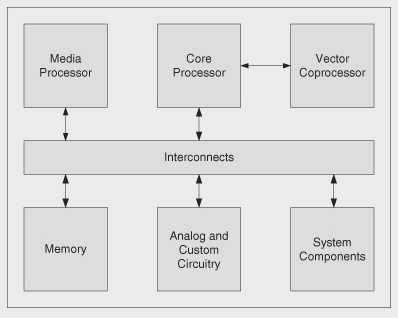
\includegraphics[scale=0.75]{imagens/basicsoc.png}\\
		{\small \textbf{Fonte:} \citeonline{MichelSoC}}
    \end{center}\label{fig:socbasic}
\end{figure}




\section{Arquitetura ARM Cortex-A9}

\subsection{Protocolo AMBA 3}

\subsection{Generic Interrupt Control - GIC}

\section{Field Programmable Gate Array - FPGA Fabric}


\section{Hardware Processos System}
% Introdução, comentar sobre a família de processadores arm
%%================================
\subsection{FPGA Manager}
\subsection{HPS-FPGA Manager}
\subsection{HPS-FPGA Bridge}
\subsection{System Interconnect}
\subsection{Cortex-A9 Microprocessor Unit Subsystem}
\subsection{DMA Controller }
\subsection{Booting}


\section{Kit de desenvolvimento DE10-nano}